% Springer Nature / Nature Portfolio compatible LaTeX submission draft.
\documentclass[pdflatex,sn-nature]{sn-jnl}

\usepackage{graphicx}
\usepackage{amsmath,amssymb,amsfonts}
\usepackage{booktabs}
\usepackage{xcolor}
\graphicspath{{figures/}}

\raggedbottom
\unnumbered

\begin{document}

\title[Bounded calibration for nutrient profiling]{Bounded attribute-level calibration for microbiome-informed nutrient profiling}

% AUTHOR_INPUT_NEEDED: Confirm the complete author list, order, affiliations,
% correspondence details, ORCID identifiers and consortium naming before
% submission. No metadata from the pre-edit dirty draft are asserted here.

\abstract{Nutrient profiling encodes food composition as population-level food-quality assessments. Individual adaptation requires a separate calibration layer around a shared population prior. The Gut Microbiome-informed Nutrient Profiling System (GMNPS) uses bounded attribute-level calibration with locked inputs. Eligible observed participant-by-meal outcomes are unavailable in the audited data, limiting the current evidence tier to computational feasibility. The locked implementation recovered the programmed mapping in a correctly specified synthetic positive-control. The framework offers an auditable computational basis for future empirical testing, while direct person-by-food response validity and clinical utility remain unestablished.}

\keywords{nutrient profiling; personalized calibration; gut microbiome; computational feasibility; synthetic positive-control}

\maketitle

\section*{Introduction}

Food-level nutrition guidance has to do two things at once. It must be stable
enough to support population advice, labelling and food-policy comparisons, yet
flexible enough to remain useful as evidence accumulates that people differ in
their metabolic responses to the same foods. Nutrient profiling systems address
the first requirement by translating food composition into a common food-quality
scale \cite{mozaffarian2021foodcompass,barrett2024foodcompass2}. Global diet
quality analyses and sustainable-diet frameworks further show why such common
scales matter for public health and food-system decisions
\cite{miller2022globaldietaryquality,willett2019eatLancet}. Precision nutrition
creates a second requirement. Deep phenotyping and challenge-meal studies have
shown substantial inter-individual variation in glycaemic, lipaemic and other
postprandial responses \cite{zeevi2015personalized,berry2020postprandial}. A
recent randomized trial further supports the translational potential of
personalized nutrition programs while underscoring the need for careful
validation \cite{bermingham2024personalized}. A nutrition score designed for
precision use therefore needs to adapt to the person without losing the shared
food ranking that makes nutrient profiling interpretable.

Current approaches tend to privilege one side of this tension. Conventional
nutrient profiling gives every person the same score for a food, so it cannot
represent person-food heterogeneity. Fully individualized recommendation models
can encode heterogeneity, but the population food-quality prior may become
implicit, weakly constrained or hard to audit. This distinction matters because
an individualized system that freely re-ranks foods may no longer function as a
nutrient profile. A precision-ready nutrient profiling framework should instead
make personalization conditional on a preserved population prior.

We use the term personalized calibration for this design. A food keeps its
baseline nutrient-profile score, and an individual receives a bounded deviation
around that score. The deviation is centered within each food and capped before
the final score is placed back on the 1 to 100 scale. This architecture converts
personalization from a replacement model into a calibration layer. It also gives
a clear validation target: the population mean should preserve the baseline
ranking, whereas individual scores should reveal structured heterogeneity that
a static score cannot express.

The gut microbiome is a plausible calibration layer because it sits at the
interface between diet, microbial metabolism and host physiology. Diet can
rapidly and reproducibly alter the gut microbiome \cite{david2014diet}, long-term
dietary patterns are associated with microbial community structure
\cite{wu2011enterotypes}, and microbiota-targeted dietary interventions can
modify immune and metabolic readouts \cite{wastyk2021microbiotaDiets}. Large
PREDICT and ZOE studies have linked microbiome features with habitual diet,
cardiometabolic markers and personalized postprandial responses
\cite{asnicar2021microbiome,fackelmann2025diet,asnicar2025gut,
segev2026dietmicrobiome}. These
studies do not imply that microbiome data alone are sufficient for clinical
dietary decisions, but they do support microbiome-informed calibration as a
biologically grounded proof of concept.

Here we introduce GMNPS as a microbiome-informed example of personalized
calibration for nutrient profiling. We use Food Compass 2.0 only as the selected
baseline prior because it provides broad, current food-attribute coverage
\cite{barrett2024foodcompass2}. The article tests whether bounded calibration
can preserve population nutrition consensus, expose person-food heterogeneity,
pass expert boundary review and behave as expected in external plausibility and
known-ground-truth simulation analyses. The central claim is deliberately
bounded: personalized calibration can make nutrient profiling more suitable for
precision nutrition, and a gut microbiome layer provides a feasible example, but
clinical efficacy and individual response prediction require further validation.

\section*{Results}

\subsection*{A bounded calibration architecture}

GMNPS was designed around a simple constraint: personalization should move a
food score only within a pre-specified neighbourhood of the population prior
(Fig.~\ref{fig:framework}). For each individual-food pair, microbiome-informed
nutrient-response features were mapped to a raw response, robustly standardized
within food, transformed through a bounded function and added to the baseline
prior. The primary cap was 12 points on the 1 to 100 scale. The final score was
therefore interpretable as a calibrated nutrient profile, not an unconstrained
recommendation score.

The personalized deviation was reported through two expert-revised channels. The
first captured microbiota-accessible carbohydrate, short-chain-fatty-acid and
plant-matrix attributes. The second captured lipid, bile-acid and
trimethylamine-N-oxide-related attributes. The two-channel reporting structure
was used for interpretability; it was not treated as direct mechanistic proof
from intervention outcomes. Expert review refined this boundary before the
primary scoring run, retaining 12 plant-matrix nutrients and 14 lipid-related
nutrients, while excluding carbohydrate from the primary channel and removing
zinc, copper and vitamin A RAE from primary microbiome-channel attribution.

\begin{figure}[t]
\centering
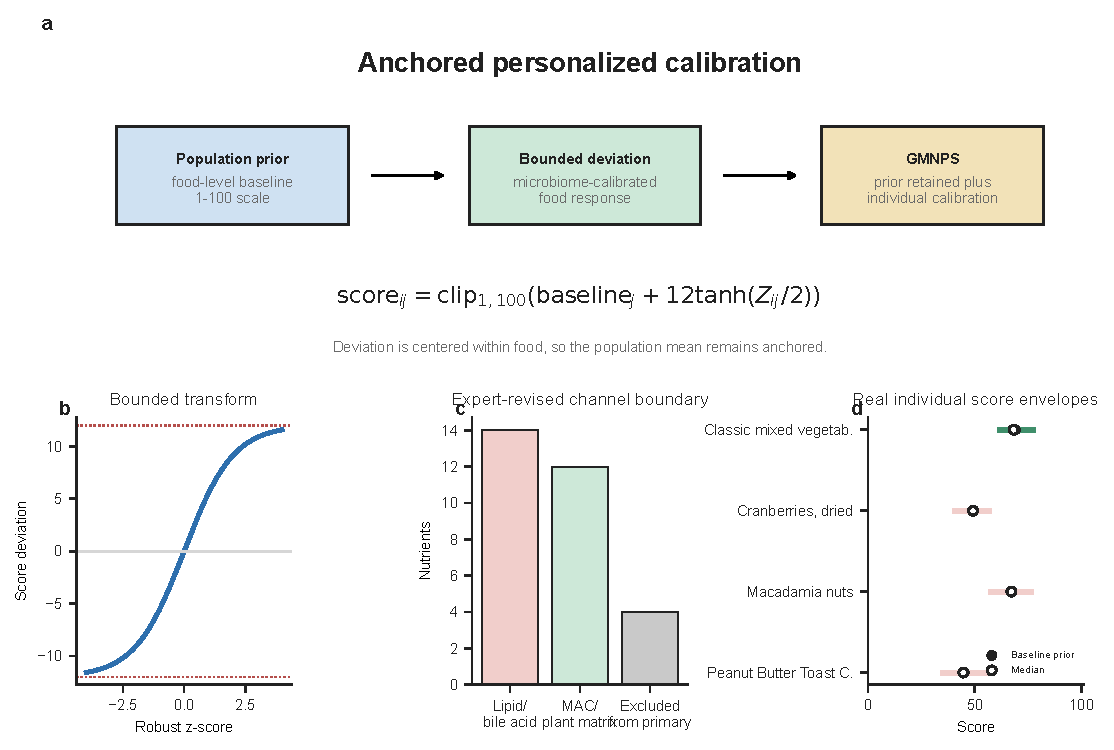
\includegraphics[width=\textwidth]{figure_1_framework.pdf}
\caption{\textbf{An anchored calibration architecture for precision-ready
nutrient profiling.} a, GMNPS adds a bounded microbiome-informed deviation to a
population food-quality prior. b, Robust individual-food responses are mapped to
a capped score deviation. c, Expert-revised channel boundaries separate
plant-matrix and lipid-related reporting features from excluded primary-channel
variables. d, Real individual score envelopes for representative foods show how
personalized values vary around the retained baseline prior. Source data are
provided with the manuscript.}
\label{fig:framework}
\end{figure}

\subsection*{Population nutrition consensus was retained}

We first asked whether personalized calibration preserved the population food
ranking. The primary run aligned baseline scores, nutrient vectors and
microbiome-derived weights for 9,234 foods and 15,492 microbiome profiles. The
population-mean GMNPS score was almost identical to the baseline prior across
foods (Spearman \(\rho=0.999839\)), exceeding the pre-specified preservation
criterion of \(\rho \geq 0.90\) (Fig.~\ref{fig:preservation}a).

Category-level behaviour showed the same pattern. Only 79 of 9,234 foods
shifted across broad category boundaries at the population mean (0.86\%).
Transitions were adjacent-boundary movements, with 38 foods moving from moderate
to minimize and 41 moving from encourage to moderate. No food moved directly
between the minimize and encourage categories (Fig.~\ref{fig:preservation}b).
Food-group means were also nearly superimposable between the baseline prior and
the calibrated population mean (Fig.~\ref{fig:preservation}c).

Bootstrap resampling of foods showed that this preservation was stable to the
composition of the scored food universe (Fig.~\ref{fig:preservation}d). The
high correlation and low category-shift rate are partly consequences of the
anchored design, and are therefore interpreted as evidence that GMNPS behaves as
a calibrated nutrient profile rather than as independent proof of clinical
validity.

\begin{figure}[t]
\centering
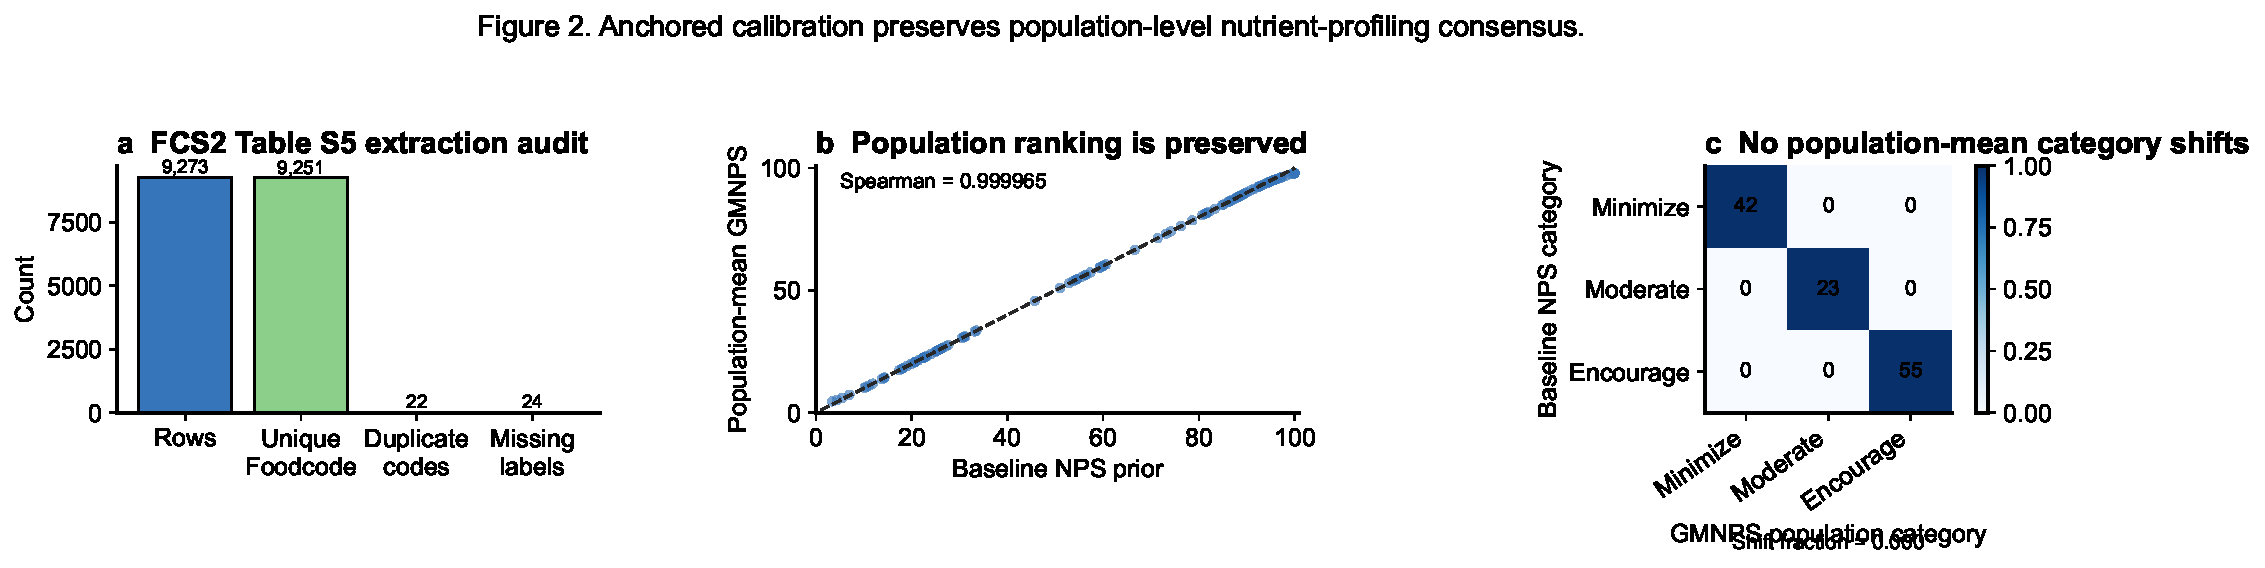
\includegraphics[width=\textwidth]{figure_2_preservation.pdf}
\caption{\textbf{Personalized calibration preserves population nutrition
consensus.} a, Baseline prior versus population-mean GMNPS across 9,234 foods.
b, Broad category transitions at the population mean. c, Food-group mean scores
for the baseline prior and calibrated population mean. d, Bootstrap
preservation estimates across resampled food universes. Source data are
provided with the manuscript.}
\label{fig:preservation}
\end{figure}

\subsection*{Calibration exposed structured person-food heterogeneity}

A static nutrient profile has no individual variance by design. GMNPS introduced
bounded variance around the preserved food-level prior. The strongest
food-level intervals remained centered near the baseline score, but individual
profiles spanned substantial ranges within the cap (Fig.~\ref{fig:heterogeneity}a).
The individual-food heat map showed that deviations were not constant across
people or foods, indicating that calibration added person-specific structure
rather than a uniform shift (Fig.~\ref{fig:heterogeneity}b).

The total variance was intentionally similar across food groups because the
bounded transform constrained the scale of personalization
(Fig.~\ref{fig:heterogeneity}c). Channel attribution, in contrast, varied by
food group. Fruit and vegetables were more often dominated by the plant-matrix
channel, whereas dairy, fats and oils, grains, meat and egg products, and
savoury or sweet foods showed larger lipid-channel contributions
(Fig.~\ref{fig:heterogeneity}d,e). These patterns are consistent with the
nutrient substrate logic of the channels, but they remain model-attributed
heterogeneity rather than measured causal effects.

\begin{figure}[t]
\centering
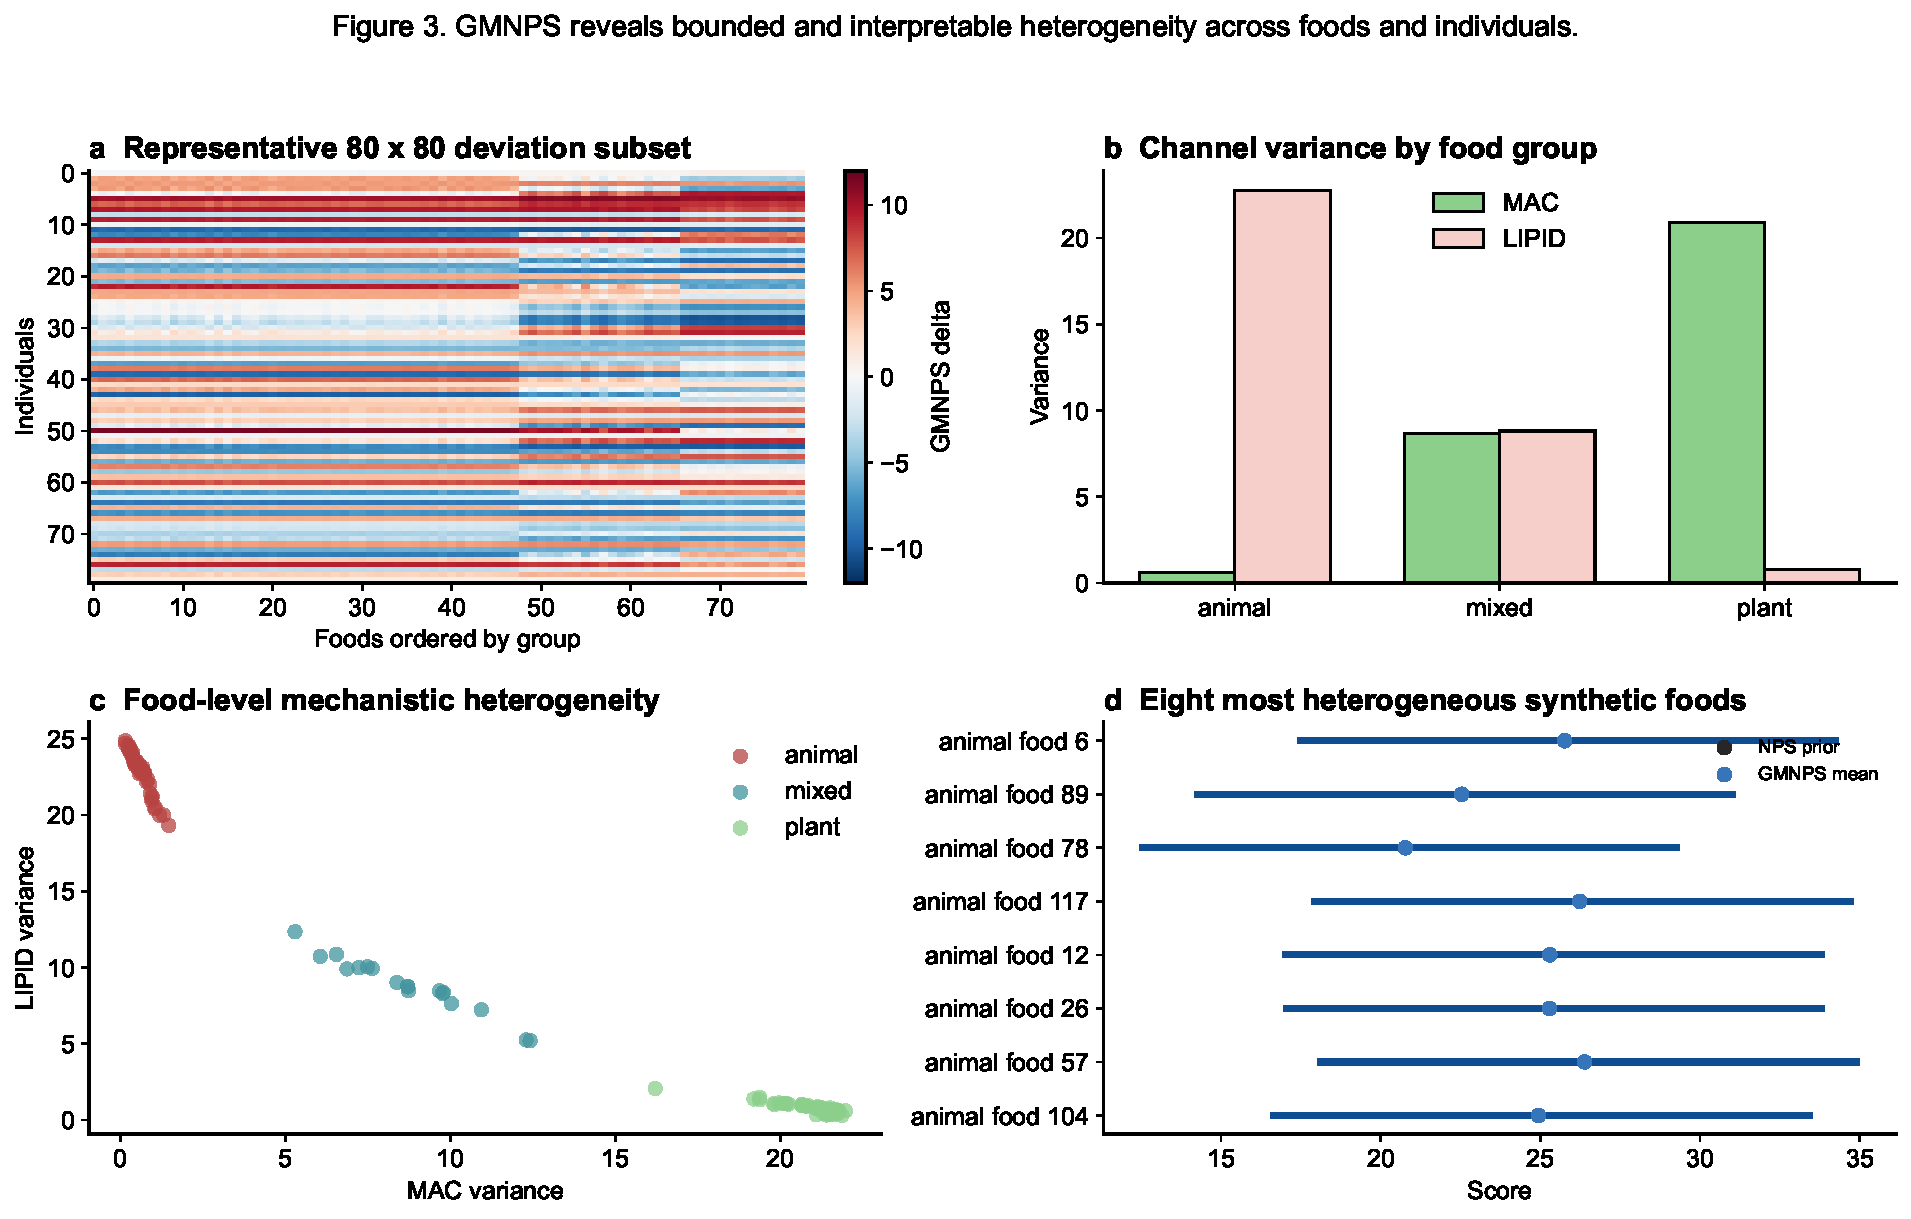
\includegraphics[width=\textwidth]{figure_3_heterogeneity.pdf}
\caption{\textbf{Calibration exposes bounded and interpretable heterogeneity.}
a, High-heterogeneity foods show broad individual score intervals while
retaining their baseline anchors. b, Individual-food deviations for 48
high-variance profiles and representative foods. c, Mean personalized variance
by food group. d, Mean plant-matrix and lipid-channel variances by food group.
e, Food-level channel dominance across the scored food universe. Source data are
provided with the manuscript.}
\label{fig:heterogeneity}
\end{figure}

\subsection*{Expert review defined the biological boundary}

We used structured expert review to define the content boundary of the
calibration layer before interpreting the primary scoring run. Six experts with
complementary backgrounds in clinical nutrition, food analysis, food bioactive
compounds, food biomarkers, population nutrition and probiotics completed two
rounds of review. The first round supported the food-group and output logic. The
second round supported the revised nutrient-channel boundary after targeted
changes. The review also noted clinical translation potential while emphasizing
that clinical application would require additional disease-stage, safety,
medication and implementation constraints.

The expert review had three direct consequences for the primary analysis.
Carbohydrate was downgraded to sensitivity or proxy use because it was too broad
to represent microbiota-accessible substrate on its own. Zinc and copper were
removed from the plant-matrix channel. Vitamin A RAE was removed from the
lipid-related channel, while retinol was retained as the more specific marker.
These revisions were used to strengthen content validity and interpretability,
not to tune model performance after observing outcomes.

\subsection*{External and simulated analyses supported plausibility and limits}

The external microbiome-health analysis was used as a plausibility check, not as
a clinical validation of food scoring. In GMrepo comparisons against healthy
controls \cite{dai2022gmrepo}, the microbiome-derived health-state component
showed modest discrimination for type 2 diabetes (AUROC 0.6332; 95\% CI,
0.6115 to 0.6528; \(n=771\) disease samples) and coronary artery disease (AUROC
0.6686; 95\% CI, 0.5823 to 0.7516; \(n=47\) disease samples)
(Fig.~\ref{fig:validation}a). Signals were weak or negative for colorectal
cancer and inflammatory bowel disease comparisons. This pattern supports a
cardiometabolic plausibility boundary and argues against presenting GMNPS as a
general disease predictor.

We then evaluated the architecture in a digital-gut-twin benchmark with known
ground truth. Across 12 repeated seeds, the baseline-only model preserved the
population ranking but had no estimable personalized residual because its
prediction did not vary by individual. Anchored GMNPS preserved the population
prior (mean \(\rho=0.9998\), s.d. 0.0001) and recovered individualized residual
structure (mean \(\rho=0.3771\), s.d. 0.0284). Random and shuffled microbiome
controls retained the prior but lost the residual signal (mean residual
\(\rho=0.0137\) and 0.0102). The unanchored microbiome score recovered some
residual structure but did not reliably preserve the population prior across
seeds (Fig.~\ref{fig:validation}b--d). Varying the deviation cap from 8 to 15
points did not materially change the preservation-residual trade-off
(Fig.~\ref{fig:validation}e). Together, these results support the central design
claim: bounded anchoring lets a personalized layer add individual signal without
collapsing the population food-quality prior.

\begin{figure}[t]
\centering
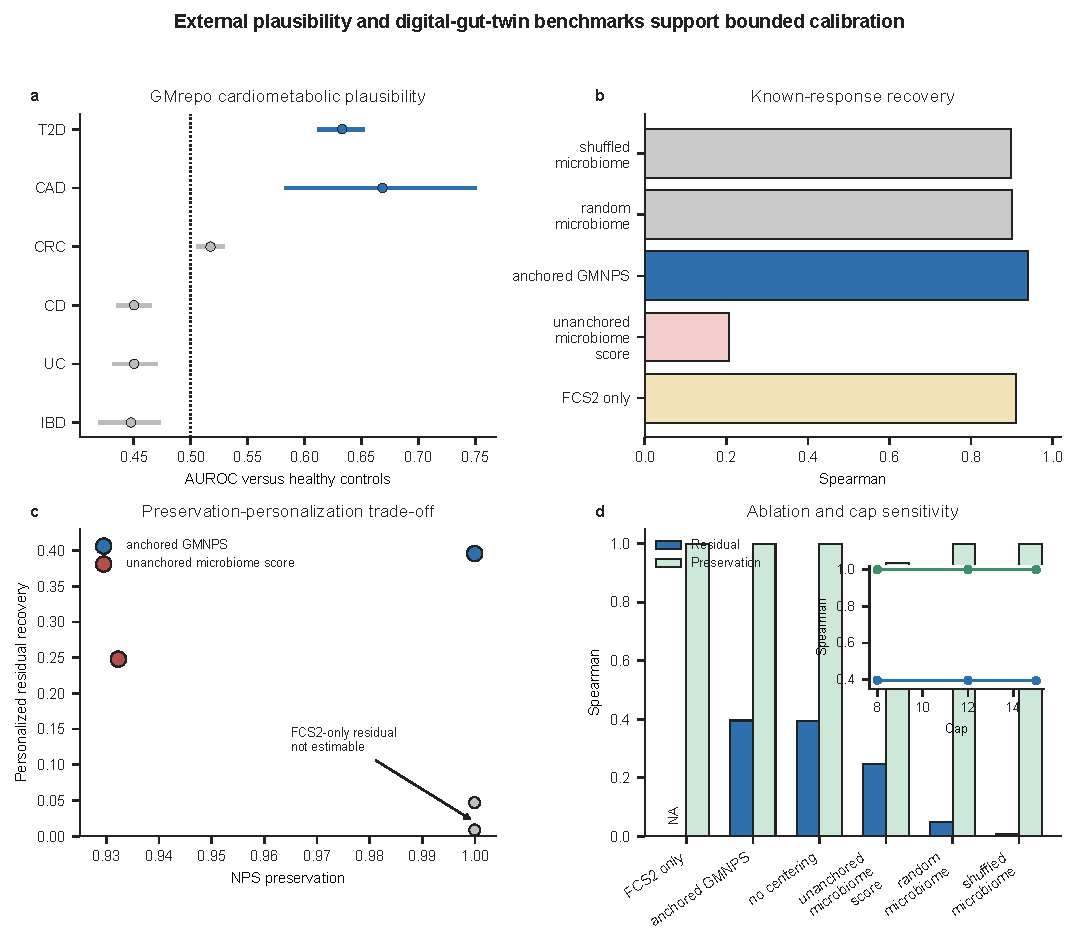
\includegraphics[width=\textwidth]{figure_4_validation.pdf}
\caption{\textbf{External plausibility and known-ground-truth benchmarks define
the validation boundary.} a, GMrepo AUROC estimates for selected disease
comparisons against healthy controls. b, Full-response recovery in repeated
digital-gut-twin runs. c, Trade-off between population-prior preservation and
personalized residual recovery. d, Architecture ablations and negative controls.
e, Sensitivity to deviation caps of 8, 12 and 15 points. Source data are
provided with the manuscript.}
\label{fig:validation}
\end{figure}

\section*{Discussion}

This study frames precision nutrition as a calibration problem for nutrient
profiling. The central advance is an architecture rather than a clinical
recommendation claim: a population food-quality prior remains explicit, while a
bounded individual-food deviation provides the space for personalization. This
design preserves the public-health role of nutrient profiling and gives
precision nutrition a controlled route for expressing heterogeneity, consistent
with the broader importance of calibration when prediction outputs are intended
to support decisions \cite{vanCalster2019calibration}.

The evidence supports three connected conclusions. First, the population mean of
GMNPS preserved the baseline food ranking across more than nine thousand foods,
with very rare category shifts. Second, the calibrated score expressed
person-food heterogeneity that a static profile cannot represent, and its
channel attribution was biologically interpretable. Third, the digital-gut-twin
benchmark showed why anchoring matters: unanchored microbiome scoring could
carry individualized signal but weakened the population prior, whereas anchored
GMNPS balanced both objectives.

The microbiome layer should be interpreted as a proof of concept. Human studies
support the gut microbiome as a link between diet quality, microbial metabolism
and host metabolic traits \cite{sanz2025gutmicrobiome,asnicar2021microbiome,
asnicar2025gut,segev2026dietmicrobiome}. The present analysis uses that biology
to define an interpretable calibration layer, but it does not prove that GMNPS
predicts clinical outcomes for a person. This boundary is important because
microbiome-diet associations are context-dependent and may be influenced by
habitual diet, medications, disease state, geography and measurement pipelines.

Several limitations follow directly from the design. The primary validation is
computational and retrospective. The GMrepo analysis tests microbiome-health
plausibility rather than food-specific response prediction. The
digital-gut-twin benchmark provides known ground truth, but simulation cannot
replace prospective or deeply phenotyped human validation. Expert review
supports channel content validity and translational relevance, not clinical
efficacy. Future evaluation should test whether calibrated deviations predict
measured postprandial or longer-term responses in datasets with matched foods,
microbiomes and host outcomes, following reporting principles for prediction
models and health AI where appropriate \cite{collins2015tripod,wolff2019probast,
liu2020consortAi}.

More broadly, GMNPS suggests a modular path for precision-ready nutrient
profiling. The baseline prior can be replaced by another well-validated nutrient
profile, and the calibration layer can incorporate microbiome, metabolomic,
continuous-glucose, genetic or clinical signals if each layer is evaluated under
the same preservation, interpretability and validation criteria. The principle
is that personalization should be visible, bounded and auditable. Under that
constraint, nutrient profiling can adapt to individual biology while retaining
its population-level purpose.

\section*{Methods}

\subsection*{Study design}

This was a computational framework and validation study. No new human
participants were recruited and no clinical intervention was conducted. The
analysis combined a baseline nutrient-profiling prior, aligned food nutrient
vectors, microbiome-derived individual weights, expert-reviewed channel masks,
external microbiome-health plausibility analysis and digital-gut-twin
simulation.

\subsection*{Baseline prior and food universe}

Food Compass 2.0 was used as the selected baseline prior because it provides
broad food-attribute coverage on a 1 to 100 scale across foods and beverages
\cite{barrett2024foodcompass2}. It was used as an anchoring prior rather than as
the focus of the contribution. The primary scoring run included 9,234 aligned
foods with baseline scores, food metadata and nutrient vectors. Nutrient files
were aligned to the Food and Nutrient Database for Dietary Studies context used
by the baseline prior.

\subsection*{Personalized calibration}

Each individual was represented by a microbiome-derived nutrient weight vector,
and each food was represented by a standardized nutrient vector. In the present
article, individual weights were treated as microbiome-derived calibration
features rather than as causal effect estimates. The reproducible pipeline
requires a sample-by-nutrient weight matrix, a food-by-nutrient matrix and
food-level metadata. Microbiome-derived weights were aligned to the nutrient
columns used for scoring, missing nutrient weights were set to zero after
column matching, and all retained samples were carried through the scoring run.

Food nutrient variables were processed before scoring to reduce dominance by
large-scale or heavy-tailed attributes. Non-negative columns with a 99th
percentile greater than 10 were log transformed with \(\log(1+x)\). Nutrients
were then winsorized at the 1st and 99th percentiles and robustly scaled by the
median and interquartile range, with scaled values clipped at four
interquartile ranges. Raw individual-food responses were computed from the
individual weights and food nutrients, robustly standardized within food, mapped
through a bounded hyperbolic tangent transform, centered and clipped to the
primary deviation cap of 12 points. The final score was clipped to the 1 to 100
scale. Sensitivity analyses used caps of 8 and 15 points.

\subsection*{Expert-reviewed channels}

The expert-revised primary mask defined two reporting channels. The
plant-matrix channel included fibre, selected carotenoids, vitamin C, food
folate, magnesium, potassium, phylloquinone and vitamin E. The lipid-related
channel included total fat, saturated fat, cholesterol, retinol, selected
saturated fatty acids, choline and vitamin B12. Carbohydrate was retained only
for sensitivity or proxy use, and zinc, copper and vitamin A RAE were excluded
from primary microbiome-channel attribution. Six experts reviewed the channel
boundary and output logic in two rounds before the primary analysis was
interpreted. The panel included one clinical nutrition expert, two food-analysis
experts, one food-biomarker expert, one population nutrition expert, one
nutrition bioactive-compound expert and one probiotics expert, with overlap in
expertise across categories. Reviewers judged whether channel assignments were
reasonable, sufficient and interpretable; disputed items were revised before
outcome interpretation. The review was not blinded and was used for content
validity, not for performance tuning.

\subsection*{Evaluation}

Population preservation was evaluated by Spearman correlation between the
baseline prior and the population-mean GMNPS score, with a pre-specified
criterion of \(\rho \geq 0.90\). Broad category shifts were counted at the
population mean. Heterogeneity was summarized by food-level variance,
individual-food intervals and channel-attributed variance. External plausibility
was assessed with GMrepo disease comparisons against healthy controls
\cite{dai2022gmrepo}. The digital-gut-twin benchmark generated synthetic
individual microbial capacities, food substrate exposures and known host
responses, following the broader use of virtual twin concepts in precision
nutrition \cite{adams2020digitaltwins}. It then compared baseline-only scoring,
unanchored microbiome scoring, anchored GMNPS, random microbiome weights,
shuffled microbiome profiles and design ablations across repeated seeds. The
article-facing repeated benchmark used seeds 42 to 53, 160 simulated individuals
and 100 simulated foods per seed. The manuscript figures were generated in
Python using pandas, NumPy and matplotlib; parquet-backed matrix extracts used
pyarrow.

\section*{Data availability}

Food Compass 2.0 scores are available from the original Food Compass 2.0 article
and supplement \cite{barrett2024foodcompass2}. FNDDS files are available from
USDA FoodData Central and USDA Food Surveys Research Group resources. Public
PREDICT/ZOE microbiome resources are available through the repositories reported
in the 2025 ZOE data availability statement \cite{asnicar2025gut}. Restricted
individual-level clinical, dietary and intervention variables require approved
access from the data holders. Figure source data are generated by the analysis
scripts and included with the manuscript package.

\section*{Code availability}

GMNPS scoring, source-data generation, synthetic benchmarking and figure
generation scripts are maintained in the project repository. Large generated
matrices and rendered outputs are reproducible from the committed scripts and
are excluded from Git by default because of file size.


\backmatter

% AUTHOR_INPUT_NEEDED: Confirm acknowledgements, funding, author contributions,
% competing interests, ethics wording and materials correspondence. These
% declarations are intentionally not rendered until confirmed by the authors.

\bibliography{references}

\end{document}
